\documentclass{standalone}

\usepackage{amsmath}
\usepackage{tikz}
\usetikzlibrary{shapes, arrows.meta, positioning, backgrounds}

\tikzstyle{block} = [rectangle, minimum width=2cm, minimum height=1cm, text centered, draw=black, fill=white]
\tikzstyle{arrow} = [->,>=stealth]

\begin{document}
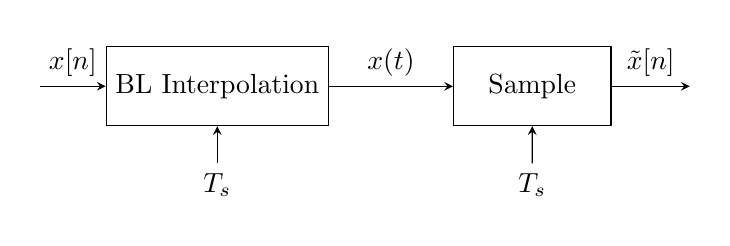
\begin{tikzpicture}[node distance=4cm, background rectangle/.style={fill=white}, show background rectangle]

    \node (block0) [block] at (0, 0) {BL Interpolation};
    \node (block1) [block, right of=block0] {Sample};
    \node (Ts0) at (0, -1.25) {$T_s$};
    \node (Ts1) at (4, -1.25) {$T_s$};

    \draw [arrow] (-2.25, 0) -- node[anchor=south] {$x[n]$} (block0);
    \draw [arrow] (block0) -- node[anchor=south] {$x(t)$} (block1);
    \draw [arrow] (block1) -- node[anchor=south] {$\tilde x[n]$} (6, 0);

    \draw [arrow] (Ts0) -- (block0);
    \draw [arrow] (Ts1) -- (block1);

\end{tikzpicture}
\end{document}